\chapter{Circuit simulations for generating various waveform signals}
% Outline the simulation results based on the chosen approach in the previous chapter
The circuit simulations are run to validate the behaviour of the conceptual design of the Riemann Pump. The simulated output signal already identifies some fundamental ideas to understand the drawbacks and trade-offs of the designed circuit.\\
To investigate the theoretical concepts of chapter \ref{ch:design} the harmonic balance simulator is used.
The harmonic balance simulation is done with the design tool \gls{ab:ads}.
The benefit of the harmonic balance simulation is that the whole system is modelled in a steady state mode, so that no transients influences the results. \textit{"Harmonic balance is a frequency-domain analysis technique for simulating non linear circuits and systems[...]"}  ADS\_Harmonic\_Balance.pdf\\
In a first step the analog signal across the output impedance in the time domain is plotted to check whether a signal could be synthesized or not. 
After various signals could be synthesized, a short stability and energy consumption analysis is done.
The stability check is needed to validate that the circuit do not oscillate.
As well the circuits energy consumption has to be checked if it is in a moderate range (\textit{which is the moderate range? mention it here?}) since it could be implemented in mobile devices.\\
    In the last step a simulation is run which makes the concept comparable to the realized circuit. 
   In this simulation the transistor dimensions are adapted to the dimension of the built demonstrator. 
   This should give an insight to the behaviour of the constructed demonstrator.\\
   It is important to note that all simulations are done under ideal conditions and hence no losses are taken into account. 
    The modelling and simulation of the designed circuit under real conditions considering all loss effects would go beyond the scope of this thesis. Therefore a keep it small and simple approach is chosen.\\   

\section{Generating various analog signals with digital input control}
The generation of analog signals at the output of the designed circuit is the purpose of this concept.
 The designed Riemann Pump should be able to create various (arbitrary) waveform signals by converting a digital bit sequence into the analog output signal.
 % Therefore the Riemann Pump is a arbitrary waveform generator and also a high speed digital-to-analog converter
%To validate the feasibility of the presented concept, a digital input control code is required.
%To get this code an approximation by hand is done since no algorithm exists which can compute this.
Simulations in time domain are required to validate the signal integrity of the synthesized signals since the output signals consist of the integration of current over time to charge a capacitor at the output.
 %Based on the idea, to integrate the current over time to charge a capacitor at the outputlinear approximation of current charging a capacitor, this would be the best way to verify its correctness.
  If the output signal is verified to be as good as wanted, a simulation in the frequency domain can show the spurious free dynamic range of the \gls{ab:dac}.\\
To synthesize a certain analog signal at the output the corresponding Riemann Code is needed.
Due to the fact that no algorithm exists which computes this Riemann Code, it is done manually.\\ 
 %The generation of the various analog output signals is based on the concept of chapter \ref{ch:design}. 
 The presented \gls{ab:dac} have a resolution of three bit and synthesizes signals with an \gls{ab:osr} of four. 
  The components used, are optimized with respect to the signal integrity. 
  The dimension of the used components are tuned while simulation to ensure the desired output signal.
  In contrast to this optimized components, chapter \ref{ch:ProofOfConceptWithExistingComponents} deals with the simulation done with real dimensions of the demonstrator components. 
  This simulation should give an insight to what is expected for the measurements.
 
\subsection{Sine wave generation in the time domain}
As known from basic signal processing lecture
%[Oppenheim, MIT, Signals and Systems Lecture \textit{http://ocw.mit.edu/resources/res-6-007-signals-and-systems-spring-2011/lecture-notes/MITRES\_6\_007S11\_lec02.pdf}]
[REF.?] the sine wave for continuous time is the elementary signal and therefore synthesized first. 
For the generation of this sine wave a corresponding Riemann Code is required which will be converted to the analog output signal.\\
This Riemann Code is generated by hand via an approximation of a sine wave with a sequence of eight different slopes.
This eight different slopes represents a three bit resolution of the \gls{ab:dac} while the sequence consists of eight sampling points which refer to the \gls{ab:osr} of four.\\
Figure \ref{fig:RiemannCodeGenerationSineWave} presents the sequence of slopes used to approximate a sine wave. 

%\begin{figure}[htb!]
%   \centering
%   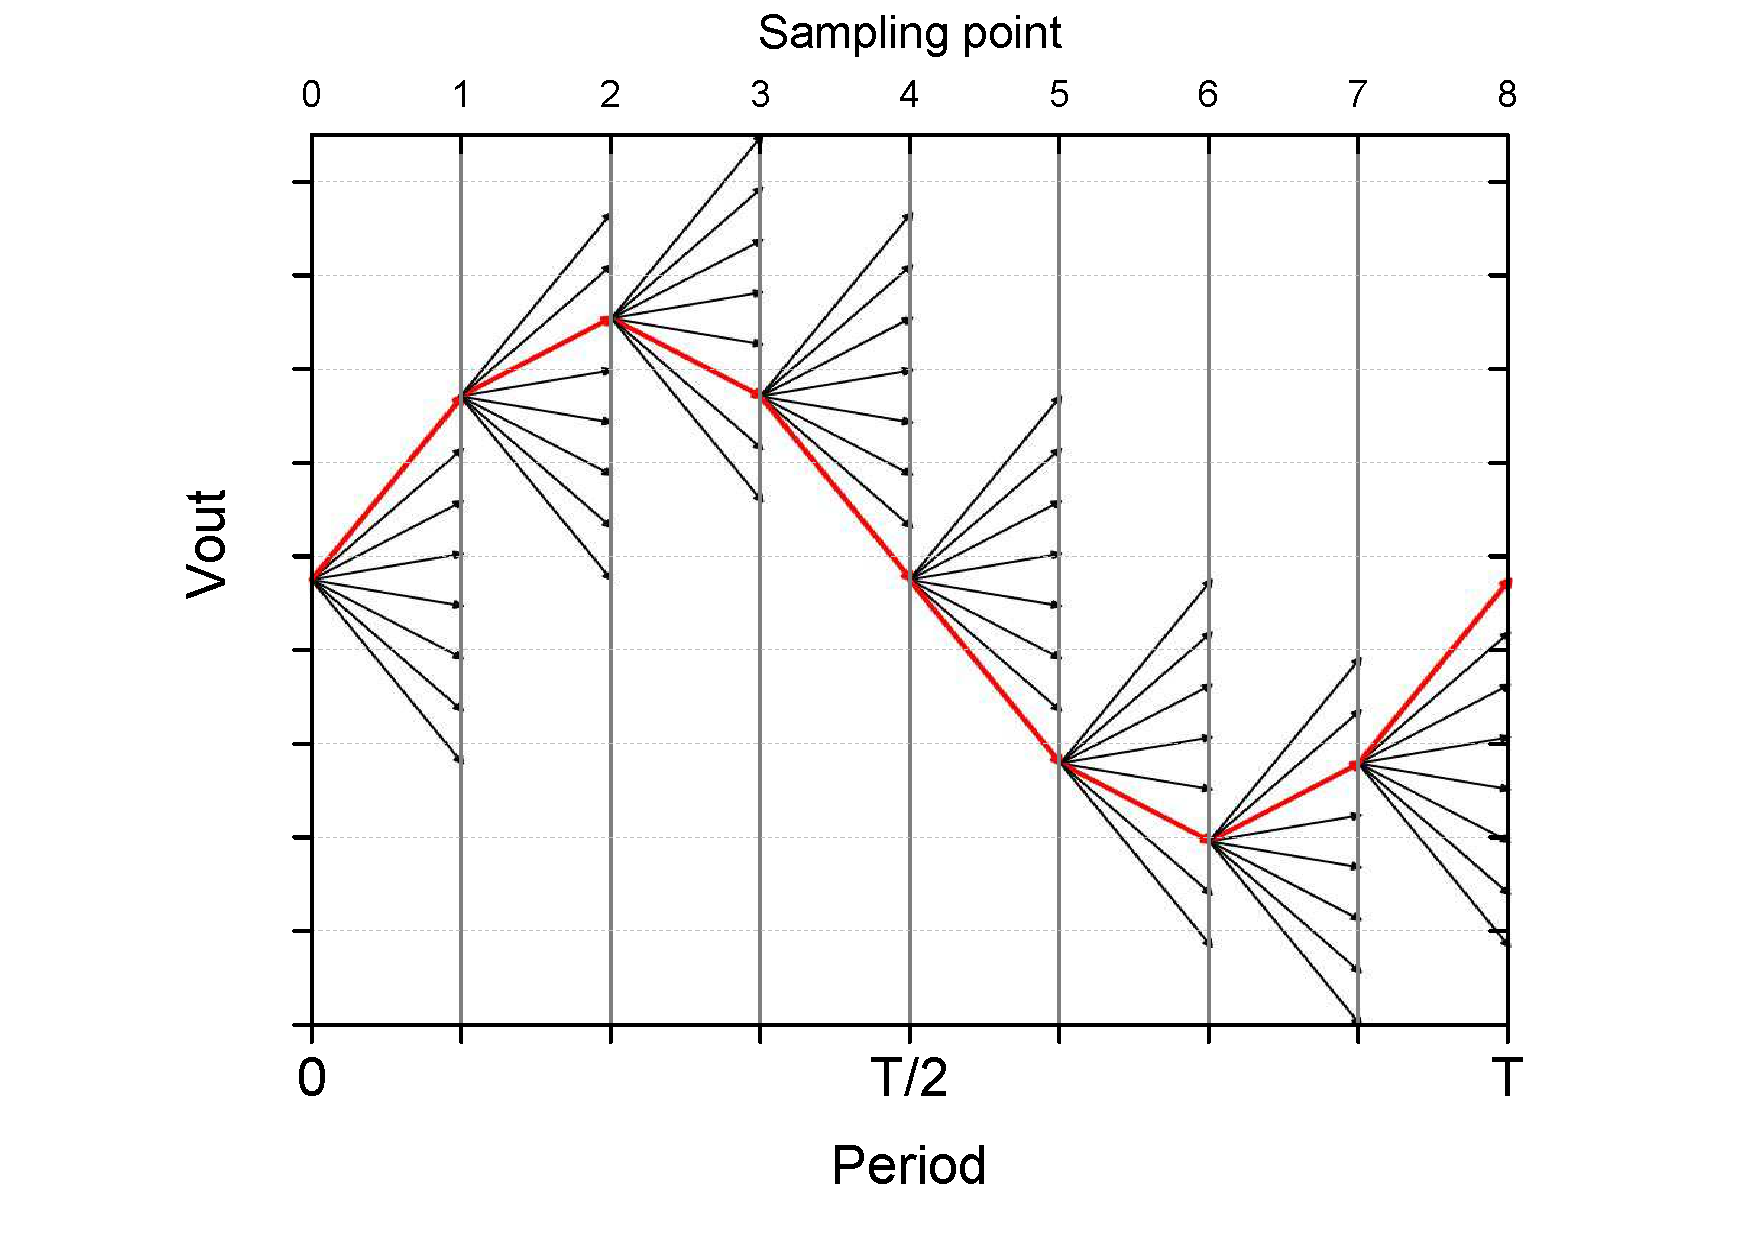
\includegraphics[width=0.75\textwidth]{RiemannCodeGeneration.pdf}
%   \caption{One possible approximation of sine wave generation to get the Riemann Code}
%   \label{fig:RiemannCodeGenerationSineWave}
%\end{figure}



\begin{figure}[htb!]
   \centering 
   \input{graphics/simulation/RiemannCodeGenerationSineWave73_latest.pdf_tex}
   \caption{One possible approximation of sine wave generation to get the Riemann Code}
   \label{fig:RiemannCodeGenerationSineWave}
\end{figure}


This sequence of slopes, referred to $i_0$ values, is:
\begin{equation}
 +7\hspace{.3cm} +3\hspace{.3cm} -3\hspace{.3cm} -7\hspace{.3cm} -7\hspace{.3cm} -3\hspace{.3cm} +3\hspace{.3cm} +7,
 \end{equation} which represents the following Riemann code:
\begin{equation}
000\hspace{.3cm} 010\hspace{.3cm} 101\hspace{.3cm} 111\hspace{.3cm} 111\hspace{.3cm} 101\hspace{.3cm} 010\hspace{.3cm} 000.
\end{equation}
\label{eq:RiemannCodeSineWave} 
   
 The Riemann Code consists of eight triplets where each triplet represent the three different switches and the number of triplets represent the number of sampling points corresponding to the \gls{ab:osr}.
This particular generated Riemann code was used to synthesize sine waves in the frequency range between \SI{500}{\MHz} and \SI{6}{\GHz}, as seen in Figure \ref{fig:7SignalsSameSlopeInOnePlot}.


\begin{figure}[htb!]
   \centering 
   \input{graphics/simulation/Vout_sine_SigBWdifferent_SameSlope_73_TwoPeriods.pdf_tex}
   \caption{Synthesized signals with demonstrated Riemann Code for the frequency range of \SI{0.5}{\GHz} .. \SI{6}{\GHz}}
   \label{fig:7SignalsSameSlopeInOnePlot}
\end{figure}

The Figure \ref{fig:7SignalsSameSlopeInOnePlot} shows seven synthesized signals generated with the same input but with different sampling frequencies. 
Here the signals amplitude is plotted over two periods in time domain.
Due to the different absolute sampling times, the amplitude of the signals differ.
The maximum reachable amplitude is the supply voltage, here set to \SI{15}{\volt} to avoid unnecessary much heat and power losses. 
If this voltage is reached, the signal wave form is clipped and transforms the sine wave into an rectangular form.
The shape from most of the plotted functions fit fairly to the one of a theoretical sine wave.
But Figure \ref{fig:7SignalsSameSlopeInOnePlot} also highlights already some limitations of the designed circuit, as the blue curve turns into a rectangular signal form.\\

\begin{figure}[htb!]
   \centering
   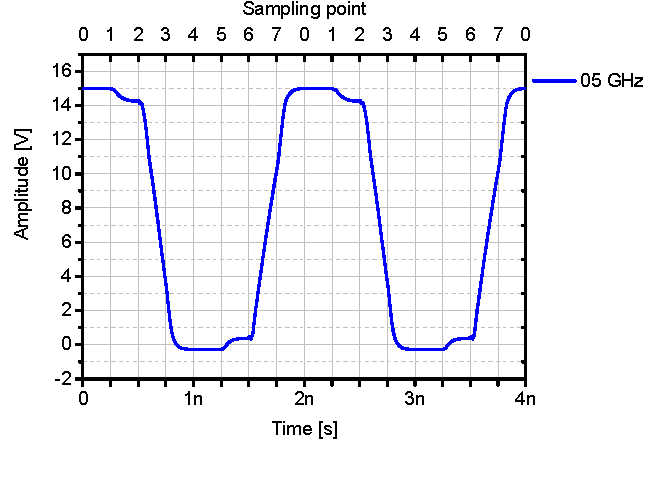
\includegraphics[width=0.75\textwidth]{Vout_sine_SigBW_05GHz_3bit_long.pdf}
   \caption{Synthesized sine wave for frequency of 0.5GHz}
   \label{fig:SineWave05GHz}
\end{figure}

The circuit designed in chapter \ref{ch:design} is optimized to cover the frequency range from \SI{1}{\GHz} to \SI{6}{\GHz} fairly well, if a voltage swing of nearly  two volts is still acceptable.
If we go beneath a frequency of \SI{1}{\GHz} the desired shape of a sine wave is going to be rectangular due to the long sampling time, refer to Figure \ref{fig:SineWave05GHz}.\\
The blue signal which should represent a sine wave with a signal frequency of \SI{500}{\MHz} is clipped and hence shows the behaviour of a rectangular signal.
 This undesired behaviour is induced from a fully charged output capacitance.
 This signal frequency is the lower bound on the frequency range for the signals for the used configuration.
%This lower bound could be shifted to even lower frequencies if the dimensions are tuned to be smaller
The upper bound on the frequency range is the signal with the at least detectable voltage swing, which could be amplified.
If at least a voltage swing of \SI{2}{\volt} is accepted, in this configuration the upper bound would be a signal frequency of \SI{6}{\GHz}.\\
% to increase this upper bound the transistor dimension have to be bigger

%%% put in the limitation here or later in a seperate paragraph???
To show how accurate the generation of the signals is, figure \ref{fig:SineWaveSynthVsTheoretical} compares a theoretical sine wave signal (red) with a synthesized one (black) for a frequency of \SI{1}{\GHz}.
The synthesized signal is same as the black curve in Figure \ref{fig:7SignalsSameSlopeInOnePlot}.
%, which within this scale already seems to turn into a rectangular signal form.
Setting up the right parameters, a good fit to a sine wave can be performed.\\
In general the sine wave is of the form: 
\begin{equation}
	v(t)= V_{DC} + \widehat{v} \cdot sin( 2  \pi  f \cdot  t + \phi).
\end{equation}
The synthesized signal (black) in Figure \ref{fig:SineWaveSynthVsTheoretical} fits pretty good to the theoretical sine wave, which has an amplitude of $\widehat{v} = \SI{7.5}{\volt}$, a signal frequency of $f = \SI{1}{\giga \hertz}$, a phase shift of $\phi = \pi / 4$ and an DC offset of $V_{DC} = \SI{7.5}{\volt}$.

\begin{figure}[htb!]
   \centering
   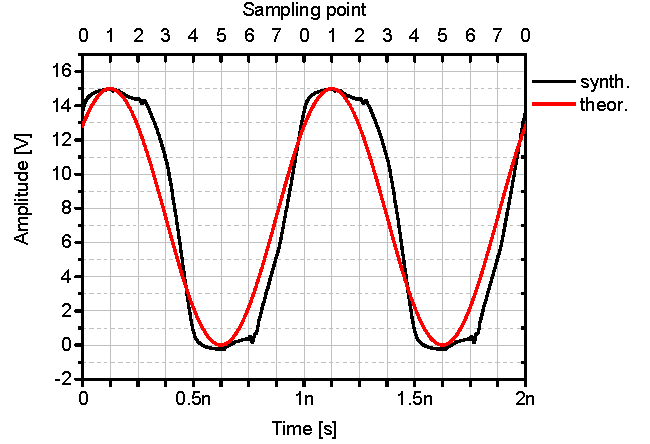
\includegraphics[width=0.75\textwidth]{Vout_SynthVsTheo.pdf}
   \caption{Synthesized sine wave with the theoretical sine wave}
   \label{fig:SineWaveSynthVsTheoretical}
\end{figure}

Although the fit seems to be very good, two distortions are visible in the peak and the valley of the synthesized signal.
($\rightarrow$\textit{Explaining these two distortions exactly for this signal frequency? Is it enough to explain some distortion at the example of 500MHz?}$\leftarrow$)
The fit is not perfect since the digital to analog conversion always introduce noise to the signal. (\textbf{refer to chapter \ref{ch:fundamentals} and the \gls{ab:sqnr}).compare to the characteristic of DAC. Which SQNR is expected, which is achieved? $\rightarrow$ plot?} \\

Figure \ref{fig:SineCompare} highlights the difference between the synthesized and the theoretical sine wave form in a more detailed way.

\begin{figure}[htb!]
	\centering
  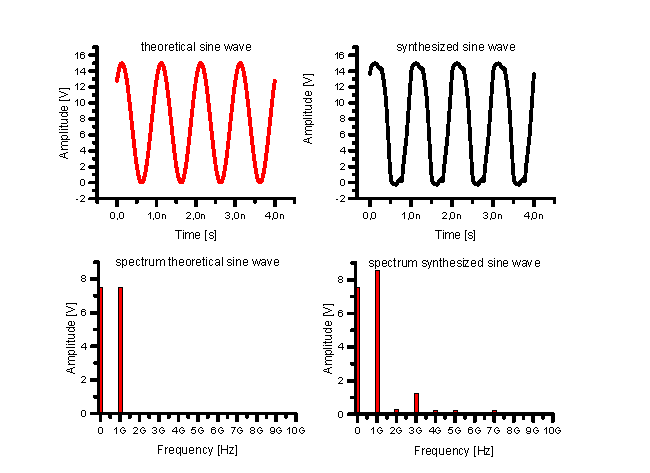
\includegraphics[width=1\textwidth]{SineCompare.pdf}
	\caption{Comparison between a theoretical and a synthesized sine wave with their spectrum}
	\label{fig:SineCompare}
\end{figure}

A sine wave is compared to the synthesized one with their corresponding spectra.
The spectra of signals are a lot easier to compare in contrast to the time domain signal with respect to the accuracy.
%The spectrum of the signal demonstrates how accurate the signal is synthesized compared to a perfectly shaped sine wave. 
Since the spectrum of a perfect sine wave only consists of a DC part and the harmonic frequency it is easy to check whether the generated signal fits to it or not.\\
On the top left side of Figure \ref{fig:SineCompare} the theoretical sine wave is plotted in red. Underneath of (the time domain signal) it the spectrum presents the frequency portion for the direct component at \SI{0} {\Hz} and a fundamental frequency portion at \SI{1}{\GHz}.
This Fourier transformation represents the frequency portions of a clear sine wave. 
The synthesized sine wave on the top right side fits fairly well to the theoretical one.
The spectrum of the synthesized signal shows nearly the same behaviour since only some harmonics distorts the signal.
Beside the direct component and the fundamental frequency component there are some additional unwanted frequency portions.
The maximum absolute distortion of this synthesized signal is about \SI{1}{\volt} in amplitude at the third harmonic at the frequency of \SI{3}{\GHz}.
 The 2nd to 10th harmonic are at most a half of a volt in absolute value of the amplitude (\textit{relative reference?}). \\
\textit{The accuracy is very good. This can be verified by the signal to noise ratio -> explain, state the SNR}


As the sampling frequency can be changed to tune the signal frequency of the output signal it is also possible to change the input control sequence to manipulate the shape of the signal.
Due to the three bit resolution there is a limited number of different slope combinations to synthesize a sine wave.
In fact there is the limit of six different combinations to synthesize the sine wave.
%For the rising edge of the upper half of sine wave, the number of slopes to synthesize is limited to two, by the fixed \gls{ab:osr} of four.
The six combination to synthesize a sine wave are: 75, 73, 71, 53, 51 ,31 with respect to the $i_0$ values.
The first digit indicates the slope of the first sampling point and the second digit respectively the second sampling point for synthesizing the rising edge of a sine wave.
%With eight different slopes representing the full spectrum between the most negative and the most positive one, exactly four slopes can represent a rising edge of a sine wave, $+7i_0, +5i_0, +3i_0, +1i_0$.
These six combinations are plotted in Figure \ref{fig:SameSigBWDifSlope} over two periods for the signal frequency of \SI{3}{\GHz}. 

\begin{figure}[htb!]
	\centering
  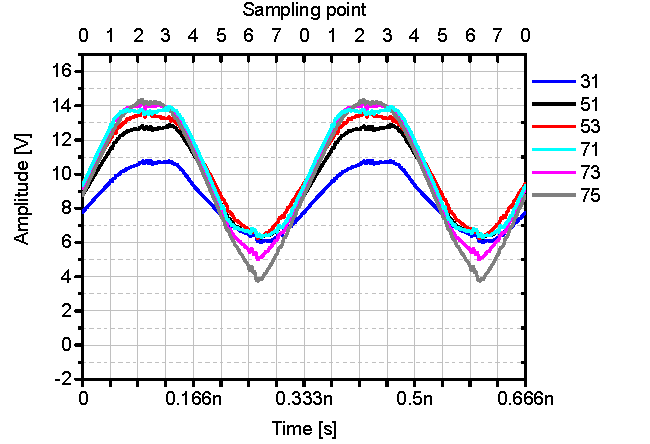
\includegraphics[width=1\textwidth]{Vout_7sine_SameSigBWdifferent_DifferentSlope.pdf}
	\caption{Signals with the same signal bandwidth but different input control}
	\label{fig:SameSigBWDifSlope}
\end{figure}

Figure \ref{fig:SameSigBWDifSlope} shows the different shapes of a sine wave for a frequency of \SI{3}{\GHz}.
This is utilized to calculate the Riemann Code which fits best to the theoretical signal.


\subsection{rectified sine wave generation in the time domain}
Based on the same approximation principle of the signal in Figure \ref{fig:SineWaveCodeGeneration}, the Riemann Code for the rectified sine is generated. 
The chosen Riemann Code for the rectified sine is:
\begin{equation}
 000\hspace{.3cm} 010\hspace{.3cm} 101\hspace{.3cm} 111\hspace{.3cm} 000\hspace{.3cm} 010\hspace{.3cm} 101\hspace{.3cm} 111.
\end{equation}
\label{eq:RiemannCodeRectSine}

Using this code a rectified sine wave is synthesized by the designed circuit.
The generation of the rectified sine wave is the same as for the normal sine wave. 
This only shows a different signal which could be synthesized.






\subsection{triangular wave generation in the time domain}
This is a triangular wave.


\section{Stability analysis of the realised circuit}
The stability and energy consumption analysis helps to get an impression/ understanding of figures and numbers of the designed circuit. Although this two aspect are of an important role for the development of a high speed \gls{ab:dac} this analysis are not complete. The whole detailed analysis could not be investigated in this thesis due to complexity and time issues, what its meaning is not to belittle. For these aspects it is important to state that the designed circuit is in no way optimized with respect to those \\
The stability analysis is important to ensure that the circuit under test do not oscillate. 
 To check this, the complex impedance at specific points in the circuit is measured.
 If the real part of the impedance is positive for the whole frequency range of the simulation, it indicates in an easy way that the circuit does not oscillate.
This simulation is done within the ADS tool. 

\section{Energy consumption analysis of the realised circuit}
If the \gls{ab:osr} is increased to get a better accuracy, the switching frequency is also increased and therefore the energy consumption.
In addition to the power consumption issue, the components have a unity current gain frequency limit.
If the resolution is increased to get a better accuracy, the whole circuit would become more complex and the energy consumption would increase.\\
Using the \gls{ab:osr} of four, we already get a sampling frequency of \SI{2}{GHz} at the lower bound.
For this reason the switches have to switch within \SI{0.5}{\nano \second} which increase the gate drive current which increase the power loss.\\
Due to the idea to use the presented topic for mobile communication it could be implemented in mobile devices, although this thesis only handles the device for the base station. If it could be used in a mobile device the energy consumption is critical.\\
The energy consumption of the designed circuit in chapter \ref{ch:design} is simulated with \gls{ab:ads}.\\
There were the trade off between the power consumption of the high side switching transistor and the switching behaviour.
Since the switching process needs to be very fast a high current is needed.
This are losses.
The driver circuit has to be optimized to reduce the energy consumption while maintaining the the switching process correctly.
If the correct hard 
\\
 For the chips used for the demonstrator refer to the work of Stephan Maroldt who states, that the power consumption is:  divided into static and dynamic ones. The switching losses are greater than the static ones.
The losses are divided into dynamic losses of the switches and static losses.
% switch voltage for on/off state, switch time, static losses and dynamic losses.

\section{Proof of concept simulation with existing components}
\label{ch:ProofOfConceptWithExistingComponents}
Simulation with ideal components but with the real dimension is done to compare with the measurement results. 

This two bit (resolution) simulation is done to compare the demonstrators measurements with the simulation. \textbf{two-bit resolution, osr = 4, keep it small and simple, frequency higher, demonstrator, assembly, less complex} 


\section{Evaluation of the simulation results for the Riemann Pump}
Nonetheless the number of signals which can be synthesized with this particular concept is increased with the possibility to change to another combination of slopes to approximate the signal.
All this calculation should be done with a signal processor and an algorithm.
With the variation of the slopes and the variation of the sampling time in theory it is possible to create every single signal with more or less good \gls{ab:sqnr}.
\\
When the component dimensions, like the switching transistors and load impedance, are fixed it is impossible to reach a bandwidth which goes from\gls{ab:dc} to \SI{6}{\GHz}.
The issue is that a small transistor dimension could synthesize signals to a very low signal frequency but will be unable to synthesize a signal at 6GHz due to the fact that the amplitude would be too small.
Hence the signal frequency bandwidth would be shifted to the smaller frequencies. 
If the \gls{ab:osr} is increased, the sampling time is decreased and therefore the signal quality is better because we have a more accurate synthesized signal. \\
If the transistor dimension is chosen to be bigger, the higher signal frequency could be synthesized with a decent voltage swing but the low signal frequencies would turn into a rectangular shape. 
This is the trade off between the shift of the bandwidth (shifting to even higher frequencies is possible but the bandwidth is nearly constant as long the output capacitance is constant too.) The trade off for the bandwidth shift to higher frequencies is, that with the signal frequency the switching frequency is increasing linearly (for an osr; eight times) and therefore the dynamic losses are increasing with this switching frequency.
By the way the transistor switching speed is determined by the dimension of the driver circuit, so if the switching speed is increased the gate driving current has to be increased to switch the transistors.

 The presented results show the theoretical feasibility of the approach.
 In a more enhanced project a MATLAB algorithm would compute this code by minimizing the deviation between a theoretical signal and the synthesized signal.
evaluate the simulation results, what is to expect in realisation. 
What is the expectation to the measurement?
